\begin{figure}[h]
    \centering
    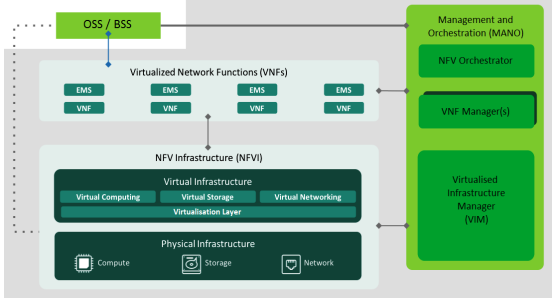
\includegraphics[width=1\textwidth]{2_2_3Architecture}
    \caption{ETSI NFV reference architecture}
    \label{fig:2_2_3Architecture}
\end{figure}

The main components of the NFV architectural framework are:\\
\\
\\
1. NFV Infrastructure (NFVI): is a kind of cloud data center containing the totality of
all hardware and software components that build up the NFV environment on which
NFV services are deployed, managed and executed. NFVI includes:

\begin{itemize}
\item \textbf{Physical Hardware:} this includes computing hardware (such as servers, RAM),
storage hardware (such as disk storage, Network Attached Storage (NAS)), and
network hardware (such as switches and routers).
\item \textbf{Virtualisation Layer:} abstracts the hardware resources and decouples the VNF
software from the underlying hardware, thus ensuring a hardware independent
lifecycle for the VNFs. We can use multiple open source and proprietary options
for the virtualisation layer (such as KVM, QEMU, VMware and Openstack).
\item \textbf{Virtual Infrastructure:} this includes virtual compute (virtual machines or containers), virtual storage, and virtual networks (overlay networks).
\end{itemize}

2. \textbf{Virtualised Network Functions (VNFs):} run on top of the NFVI and represent virtualized instances of different network functions. Each VNF has a corresponding Element Management System (EMS) that provides management and control functionality for that VNF.

3. \textbf{NFV Management and Orchestration (MANO):} NFV MANO does not act in isolation. It interacts with the Operational and Business Support Systems (OSS/BSS)
components of the operator to manage the operational and business aspects of the
network. MANO includes:

\begin{itemize}
\item \textbf{Virtualized Infrastructure Manager (VIM):} or cloud management software, e.g.
OpenStack or Kubernetes. It is responsible for controlling and managing the
computing, storage, and network resources, as well as their virtualization.
\item \textbf{VNF Manager(s):} it is responsible for VNF life cycle management, including
VNF instantiation, update, query, scaling, and termination.
\item \textbf{NFV Orchestrator:} it is in charge of the orchestration and management of NFV
infrastructure and software resources, and realizing network services on NFVI.
It utilizes resource allocation and placement algorithms to ensure optimal usage
of both physical and software resources.
\end{itemize}